\documentclass[sigconf,authorversion,nonacm]{acmart}

\usepackage{listings}

\AtBeginDocument{%
  \providecommand\BibTeX{{%
    \normalfont B\kern-0.5em{\scshape i\kern-0.25em b}\kern-0.8em\TeX}}}

\begin{document}

\title{Tarea 1 \\ Optimización ciega}

\author{Mario Emilio Jiménez Vizcaíno}
\email{A01173359@itesm.mx}

\maketitle

\section{Introducción}
Durante esta década la cantidad de datos generados por las personas y capturados por los dispositivos que usamos diariamente ha crecido exponencialmente, más rápido que la velocidad de los procesadores. Es por eso que los métodos de aprendizaje automático han tomado un papel fundamental en el procesamiento de estos, ya que estos están limitados por el tiempo de cálculo y no por el tamaño de la muestra de datos.

Los algoritmos de optimización como el gradiente descendente estocástico muestran un rendimiento sorprendente para los problemas a gran escala, ya que en promedio tienen un tiempo de ejecución mucho menor que otros algoritmos.

En esta práctica se demuestran 3 tipos variaciones de algoritmos de optimización ciega, además de sus respectivas implementaciones en Python.


\section{Metodología}
Para la demostración de los diferentes algoritmos de mutación se utilizó la búsqueda aleatoria del mínimo en la función Ackley, cuya fórmula general es:

$$f(x) = -a \exp \left(-b \sqrt{\frac{1}{d} \sum_{i=1}^{d} x_i^2} \right) -\exp \left(\frac{1}{d} \sum_{i=1}^{d} \cos (c x_i) \right) + a + \exp (1)$$

Esta función es usada frecuentemente para probar algoritmos de optimización ya que alrededor del punto mínimo global (la coordenada (0, 0)) la gráfica presenta muchos puntos mínimos locales, por lo que los algoritmos de optimización corren el riesgo de quedarse atrapados en uno de estos. En la siguiente imagen se presenta el comportamiento de esta función en dos dimensiones:

\begin{figure}[H]
  \centering
  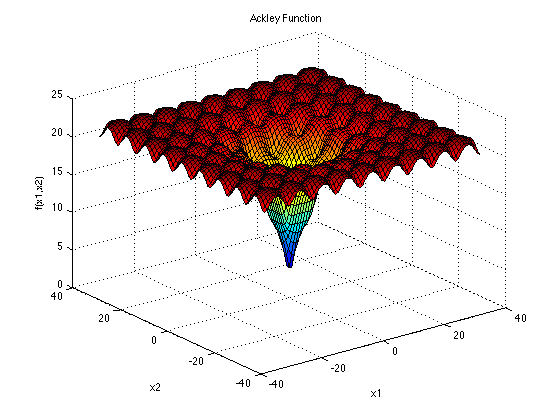
\includegraphics[width=\linewidth]{ackley.png}
\end{figure}

En este caso se usó la fórmula con dos dimensiones:

$$f(x) = -a \exp \left(-b \sqrt{\frac{x_1^2 + x_2^2}{d}} \right)$$
$$-\exp \left(\frac{\cos (c x_1) + \cos (c x_2)}{d} \right) + a + \exp (1)$$

Esta función fue evaluada en el rango $x_1, x_2 \epsilon [-32.768, -32.768]$ con los parámetros $a = 20$, $b = 0.2$ y $c = 2\pi$, utizando tres algoritmos de mutación, descritos a continuación.

La implementación de la fórmula puede ser encontrada en el apéndice B.

\subsection{Un padre, varios hijos}
La primer variante de algoritmos de mutación se llama "un padre, varios hijos" ya que en cada iteración se preserva sólo un punto (el padre), el cual se muta una cantidad predeterminada de veces para producir los hijos, de los cuales sólo el que tiene la mejor evaluación es conservado para la siguiente iteración del algoritmo.

La implementación de este algoritmo se encuentra en el apéndice C.

\subsection{Varios padres, varios hijos}
La segunda variante de mutación cambia en el número de puntos que se conservan después de cada iteración, ya que en este se conservan dos o más. Durante la mutación de padres para generar nuevos hijos se seleccionan $m$ veces un padre al azar, para mutarlo y crear un nuevo hijo. Al final, de la lista de $m$ hijos generados se seleccionan los nuevos padres para la siguiente iteración.

La implementación de este algoritmo se encuentra en el apéndice D.

\subsection{Varios padres, varios hijos, con traslape generacional}
Finalmente, esta última variante del algoritmo de mutación es muy parecida a la anterior, pero cambia en que en el último paso, la selección de nuevos padres para la siguiente iteración, se seleccionan padres de la lista de padres e hijos.

La implementación de este algoritmo se encuentra en el apéndice E.

\vfill
\pagebreak

\section{Resultados}
Para cada variante del algoritmo de mutación se creó una clase que iteraba 50 veces, generando 10 hijos en el algoritmo de un padre, varios hijos, y conservando 10 hijos en los algoritmos de varios padres, varios hijos. El código de inicio ejecutó el experimento 10 veces para calcular un promedio y una desviación estándar de estas iteraciones, para finalmente crear una gráfica del progreso del algoritmo al encontrar el punto mínimo global.

\subsection{Un padre, varios hijos}
\begin{figure}[H]
  \centering
  \includegraphics[width=\linewidth]{upvh.png}
\end{figure}

En esta primera gráfica se puede observar que muchos de los experimentos variaron demasiado entre las iteraciones 10 y 30, pero después la mayoría encontró el mínimo global de la función.

\subsection{Varios padres, varios hijos}
\begin{figure}[H]
  \centering
  \includegraphics[width=\linewidth]{vpvh.png}
\end{figure}

En el segundo algoritmo, muchos de los experimentos encontraron rápidamente el mínimo global, aunque probablemente un par de ellos no haya llegado tan rápido, provocando el aumento de la desviación estándar hasta el final.

\pagebreak

\subsection{Varios padres, varios hijos, con traslape generacional}
\begin{figure}[H]
  \centering
  \includegraphics[width=\linewidth]{vpvht.png}
\end{figure}

Finalmente, este algoritmo, a pesar de que debería ser un poco mejor que el anterior tuvo un rendimiento comparable con éste, al igual conservando un poco de desviación estándar hasta el final de las 50 iteraciones.


\section{Conclusión}
En esta práctica se demostró la utilidad y una implementación de algunos de los algoritmos de mutación, además de los resultados que podríamos esperar al seleccionar uno de estos. También se mostró que los algoritmos con traslape generacional, a pesar de tener buenos fundamentos teóricos ya que permiten que los padres que tuvieron una muy buena evaluación sean seleccionados para la siguiente iteración, a veces puede ser preferible un algoritmo de mutación sin traslape para así generar más hijos que implementen mutaciones que probablemente sean beneficiosas para avanzar en la optimización del problema.


\clearpage

\appendix

\lstset{
  frame=single,
  basicstyle=\footnotesize,
  numbers=left,
  numbersep=5pt,
  showstringspaces=false
}

\begin{figure*}
  \section{Código de entrada para los tres algoritmos}
  \lstinputlisting[language=Python]{main.py}
\end{figure*}

\begin{figure*}
  \section{Implementación de la función Ackley para una lista $[x_1, x_2]$}
  \lstinputlisting[language=Python]{AckleyFunction.py}
\end{figure*}

\begin{figure*}
  \section{Implementación del algoritmo de mutación "Un padre, varios hijos"}
  \lstinputlisting[language=Python]{UP_VH.py}
\end{figure*}

\begin{figure*}
  \section{Implementación del algoritmo de mutación "Varios padres, varios hijos"}
  \lstinputlisting[language=Python]{VP_VH.py}
\end{figure*}

\begin{figure*}
  \section{Implementación del algoritmo de mutación "Varios padres, varios hijos, con traslape generacional"}
  \lstinputlisting[language=Python]{VP_VH_T.py}
\end{figure*}


\end{document}
\endinput